\subsubsection{Aplikace IndoorCO2Map}

Čtvrtou analyzovanou aplikací je německá aplikace \textit{IndoorCO2Map}, jejímž autorem je Aurel Wünsch z Lipska. Na rozdíl od ostatních analyzovaných aplikací, které se zaměřují primárně na monitorování vnějšího prostředí, je \textit{IndoorCO2Map} orientována výhradně na vnitřní prostředí veřejně přístupných budov, jako jsou obchody, restaurace, školy, nemocnice či prostředky veřejné dopravy. Projekt se skládá z mobilní aplikace pro sběr dat (Android a iOS) a webového rozhraní pro jejich vizualizaci. Měřenou veličinou je výhradně koncentrace CO\textsubscript{2} v jednotkách ppm. \parencite{IndoorCO2MapCO2Monitoring2024}

Zdrojový kód mobilní aplikace je k dispozici ve dvou verzích: starší V1 pod licencí MIT \parencite{aurelwuAurelWuIndoorCO2AppMAUI2026} a novější V2 pod licencí GPLv2 \parencite{aurelwuAurelWuIndoorCO2MapApp2026}. Nasbíraná data jsou publikována pod licencí CC0 1.0 Universal (Public Domain), což umožňuje jejich volné využití bez jakýchkoli omezení \parencite{zotero-item-571}.

Na rozdíl od ostatních aplikací, u nichž je přehled sledovaných veličin shrnut v samostatné tabulce, u aplikace \textit{IndoorCO2Map} není tabulka veličin účelná, neboť aplikace měří výhradně koncentraci CO\textsubscript{2}. Žádné další veličiny relevantní pro IEQ (teplota, relativní vlhkost, koncentrace mikročástic, hladina hluku, osvětlenost apod.) nejsou sbírány ani přenášeny na backend. Některé podporované senzory (např. Airvalent) sice hardwarově měří i teplotu, avšak aplikace tyto hodnoty neextrahuje \parencite{aurelwuAurelWuIndoorCO2MapApp2026}. Na webovém rozhraní je z naměřených hodnot CO\textsubscript{2} odvozováno tzv. GO IAQS skóre na stupnici 0--10, které slouží jako zjednodušený indikátor kvality vnitřního vzduchu \parencite{IndoorCO2Atlas}.

Data z aplikace \textit{IndoorCO2Map} jsou přístupná dvěma způsoby. Aplikace neposkytuje žádné veřejné REST ani jiné API pro čtení dat. Webové rozhraní nenačítá data z API, ale ze statického předgenerovaného JSON souboru. Existuje pouze interní API pro zápis dat z mobilní aplikace, které odesílá měření prostřednictvím HTTPS POST požadavků na cloudovou infrastrukturu Amazon Web Services (AWS) \parencite{aurelwuAurelWuIndoorCO2MapApp2026}.

Prvním způsobem přístupu k datům je \textit{archiv dat} ke stažení.\footnote{\url{https://indoorco2map.com/chartdata/IndoorCO2MapData.zip}} Je k dispozici ZIP archiv obsahující kompletní datovou sadu ve formátu JSON (19\,720 záznamů v~době stažení), soubor s licencí CC0 1.0 Universal a popis datových polí. Každý záznam obsahuje typ a identifikátor prvku z OpenStreetMap (OSM), název lokality, GPS souřadnice, kód země dle ISO 3166-1 alpha-3, NUTS\,3 region, OSM klíč a tag, začátek měření ve formátu ISO 8601, informace o otevřených oknech a ventilaci, pole hodnot CO\textsubscript{2} v~ppm, interval měření a průměrnou hodnotu CO\textsubscript{2} \parencite{zotero-item-571}.

Druhým způsobem je \textit{webové rozhraní} na adrese \href{https://indoorco2map.com}{indoorco2map.com}, které zobrazuje nasbíraná data na interaktivní mapě (viz obrázek č.~\ref{obr:indoorco2map-map}). Data jsou načítána z~předgenerovaného komprimovaného JSON souboru, nikoli z~API v~reálném čase. Jednotlivé body na mapě představují konkrétní místa měření a jsou barevně odlišeny podle dosaženého GO IAQS skóre. Po kliknutí na vybraný bod se zobrazí detail měření včetně grafu průběhu koncentrace CO\textsubscript{2} v~čase. Webové rozhraní disponuje sadou filtrů (viz obrázek č.~\ref{obr:indoorco2map-filters}), které umožňují omezit zobrazená data podle názvu lokality, země, typu lokality odvozeného z~OSM tagů (např. supermarket, škola, nemocnice), časového rozsahu a rozsahu GO IAQS skóre. Součástí panelu filtrů je histogram distribuce lokací podle průměrné koncentrace CO\textsubscript{2} v~aktuálně vyfiltrované oblasti (viz obrázek č.~\ref{obr:indoorco2map-filters-histogram}). Prostřednictvím navigačního menu (viz obrázek č.~\ref{obr:indoorco2map-menu}) má uživatel přístup k~dalším analytickým pohledům, jako jsou souhrnné statistiky měření podle typu lokality, statistiky aktivity měření podle regionů NUTS\,1, zobrazení prostředků veřejné dopravy na samostatné mapě či možnost stažení dat odpovídajících aktuálnímu výběru \parencite{IndoorCO2Atlas}.

\begin{figure}[htbp!]\centering
\caption{Webové rozhraní aplikace IndoorCO2Map}
\label{obr:indoorco2map-map}
\includegraphics[width=.90\textwidth]{img/indoorco2map-map}

\footnotesize \textit{Poznámka:} 1 - konkrétní místo měření, 2 - zobrazení detailu průběhu měření, 3 - interpretace úrovně CO\textsubscript{2} pomocí GO IAQS skóre a barvy, 4 - filtry zobrazení.

\footnotesize \textit{Zdroj:} Snímek obrazovky pořízen autorem z webového rozhraní aplikace \parencite{IndoorCO2Atlas}.
\end{figure}

\begin{figure}[htbp!]\centering
\caption{Filtry webového rozhraní aplikace IndoorCO2Map}
\label{obr:indoorco2map-filters}
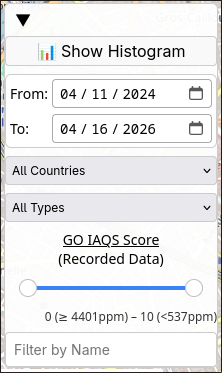
\includegraphics[width=.70\textwidth]{img/indoorco2map-filters}

\footnotesize \textit{Poznámka:} Od shora dolů: Zobrazení histogramu momentálního filtru (včetně hranice náhledu), filtrování dle časového rozsahu, filtrování dle země, filtrování dle typu lokality (restarace, škola, apod.), filtrování dle koncentrace CO\textsubscript{2} (GO IAQS skóre), filtrování podle názvu měření. 

\footnotesize \textit{Zdroj:} Snímek obrazovky pořízen autorem z webového rozhraní aplikace \parencite{IndoorCO2Atlas}.
\end{figure}

\begin{figure}[htbp!]\centering
\caption{Histogram distribuce CO\textsubscript{2} filtrované oblasti v aplikaci IndoorCO2Map}
\label{obr:indoorco2map-filters-histogram}
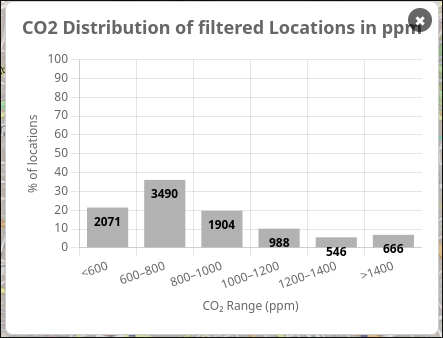
\includegraphics[width=.70\textwidth]{img/indoorco2map-filters-histogram}

\footnotesize \textit{Poznámka:} Histogram zobrazuje distribuci lokací v aktuálním filtru podle jejich průměrné koncentrace CO\textsubscript{2} v ppm.

\footnotesize \textit{Zdroj:} Snímek obrazovky pořízen autorem z webového rozhraní aplikace \parencite{IndoorCO2Atlas}.
\end{figure}

\begin{figure}[htbp!]\centering
\caption{Menu se zájmovými metrikami v aplikaci IndoorCO2Map}
\label{obr:indoorco2map-menu}
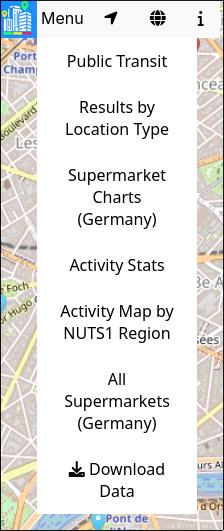
\includegraphics[width=.50\textwidth]{img/indoorco2map-menu}

\footnotesize \textit{Poznámka:} Metriky od shora: 1 - Metriky z prostorů veřejné dopravy, 2 - statistika měření pro každý typ lokace (restaurace, škola, apod.), 3 - statistika měření pro německé supermarkety, 4 - statistika aktivity měření, 5 - statistika aktivity měření podle NUTS1 regionu, 6 - zobrazní všech německých supermarketů na mapě včetně těch, které žádné měření neposkytnuly, 7 - stažení dat aktuálního náhledu 

\footnotesize \textit{Zdroj:} Snímek obrazovky pořízen autorem z webového rozhraní aplikace \parencite{IndoorCO2Atlas}.
\end{figure}


V tabulce č.~\ref{tab:indoorco2map-supported-sensors} je uveden přehled senzorů podporovaných aplikací \textit{IndoorCO2Map} a veličin, které tyto senzory hardwarově měří. Aplikace podporuje přesně čtyři modely CO\textsubscript{2} monitorů komunikujících přes rozhraní Bluetooth Low Energy (BLE); uživatel nemůže přidat vlastní typ senzoru \parencite{aurelwuAurelWuIndoorCO2MapApp2026}.

\begin{table}[!tbp]
  \centering
  \footnotesize
  \setlength{\tabcolsep}{2pt}
  \renewcommand{\arraystretch}{1.1}
  \caption{Podporované senzory IndoorCO2Map a jejich měřené veličiny relevantní pro IEQ}
  \label{tab:indoorco2map-supported-sensors}
  \begin{tabular}{l@{\hspace{12pt}}*{8}{c}@{\hspace{12pt}}*{3}{c}@{\hspace{12pt}}*{2}{c}@{\hspace{12pt}}*{2}{c}}
    \toprule
    \multirow{3}{*}{\textbf{Senzor}} & \multicolumn{15}{c}{\textbf{Kategorie IEQ}} \\
                                     & \multicolumn{8}{c}{\textbf{IAQ}} & \multicolumn{3}{c}{\textbf{TK}} & \multicolumn{2}{c}{\textbf{SK}} & \multicolumn{2}{c}{\textbf{AK}} \\
                                     & PM\textsubscript{2.5} & PM\textsubscript{10} & O\textsubscript{3} & NO\textsubscript{2} & SO\textsubscript{2} & CO & CO\textsubscript{2} & TVOC & $T$ & RH & $v$ & $E$ & CCT & $L_A$ & $L$ \\
                                     \hline
Aranet4 &  &  &  &  &  &  & \cmark &  & \cmark & \cmark &  &  &  &  &  \\
\hline
Airvalent &  &  &  &  &  &  & \cmark &  & \cmark & \cmark &  &  &  &  &  \\
\hline
AirSpot Health &  &  &  &  &  &  & \cmark &  & \cmark & \cmark &  &  &  &  &  \\
\hline
Inkbird IAM-T1 &  &  &  &  &  &  & \cmark &  & \cmark & \cmark &  &  &  &  &  \\
    \bottomrule
  \end{tabular}

  \footnotesize \textit{Zdroj:} Vlastní zpracování na základě \parencite{Aranet4HOMEIndoor, PremiumBlackAirvalent, AirSpot, INKBIRDWireless4in1}.
\end{table}

Všechny podporované senzory jsou dedikované CO\textsubscript{2} monitory využívající měřicí princip nedisperzní infračervené absorpce (NDIR) a vedle koncentrace CO\textsubscript{2} měří rovněž teplotu a relativní vlhkost \parencite{Aranet4HOMEIndoor, PremiumBlackAirvalent, AirSpot, INKBIRDWireless4in1}. Aplikace \textit{IndoorCO2Map} však z~těchto senzorů extrahuje a odesílá na backend výhradně hodnoty CO\textsubscript{2}; teplota ani vlhkost nejsou přenášeny \parencite{aurelwuAurelWuIndoorCO2MapApp2026}. Pro každý senzor existuje ve zdrojovém kódu aplikace samostatná implementace, což znamená, že aplikace je přímo závislá na konkrétním hardwaru \parencite{aurelwuAurelWuIndoorCO2MapApp2026}.

Tento přístup se zásadně odlišuje od ostatních analyzovaných aplikací. Zatímco u aplikací Sensor.Community a openSenseMap uživatel připojuje senzor k mikrokontroléru a buduje senzorovou stanici, u \textit{IndoorCO2Map} uživatel používá komerční CO\textsubscript{2} monitor spárovaný přes BLE s mobilním telefonem. Lokalizace měřeného místa rovněž nevychází přímo od uživatele — aplikace využívá OSM Overpass API k vyhledání nejbližších budov v okolí a uživatel vybírá z nabízených OSM objektů \parencite{aurelwuAurelWuIndoorCO2MapApp2026, IndoorCO2MapCO2Monitoring2024}.

Z hlediska technické architektury je mobilní aplikace multiplatformní (Android, iOS). Sběr dat probíhá v řetězci: BLE senzor odesílá data do mobilního telefonu, který je následně přenáší prostřednictvím HTTPS POST požadavku ve formátu JSON na AWS API Gateway. Backend je postaven na serverless architektuře AWS; konkrétní databáze není veřejně dokumentována. Webový frontend je implementován jako statické HTML s JavaScriptem. Aplikace podporuje dva režimy měření: měření v budově (\textit{Building}) a měření ve veřejné dopravě (\textit{Transit}) \parencite{aurelwuAurelWuIndoorCO2MapApp2026}.
